\chapter{算符、可觀測量與泡利矩陣}

好的記號不是裝飾。在一門以抽象向量和複數為基礎的學科中，若記號能讓我們直接運算符號，不必一再把它們轉成文字，本身就是不可或缺的工具。狄拉克的左矢--右矢記號之所以有用，正是因為它能讓態空間的幾何結構清晰可見，同時又便於我們利用分量和矩陣計算。

我們眼前要處理的是數學問題。我們將引入線性算符，了解它們如何作用於左矢和右矢，並辨明稱為厄米算符的特殊類別。之後才會引入\emph{可觀測量}、\emph{測量結果}和\emph{機率}這些物理概念。這樣一來，三個自旋可觀測量便會自然地以泡利矩陣的形式出現，而不是成為要死記的對象。

\section{正交歸一基底與分量}

態構成一個複數線性向量空間，其中的右矢可以相加，也可以乘以複數。每個右矢\(\ket{A}\)都有一個相應的左矢\(\bra{A}\)，由共軛對偶運算得到。基底並不唯一；但選定基底後，每個向量都能以其在該基底中的分量表示。

令
\[
\bigl\{\ket{1},\ket{2},\ldots,\ket{N}\bigr\}
\]
為一組正交歸一基底。正交性與歸一條件可合寫為
\begin{equation}
\braket{j}{i}=\delta_{ji}.
\label{eq:orthonormal-basis}
\end{equation}
當\(j=i\)時，\(\delta_{ji}\)為1；否則為0。空間的維度\(N\)是其中彼此正交的方向數目上限；一組完備的正交歸一基底恰好包含這麼多個向量。

將任意右矢展開為
\begin{equation}
\ket{A}=\sum_i \alpha_i\ket{i}.
\label{eq:ket-expansion}
\end{equation}
這些係數並不神秘。從左側乘上\(\bra{j}\)：
\begin{align}
\braket{j}{A}
 &=\sum_i\alpha_i\braket{j}{i} \\
 &=\sum_i\alpha_i\delta_{ji}
 =\alpha_j.
\end{align}
因此
\begin{equation}
\alpha_i=\braket{i}{A}.
\label{eq:components-inner-products}
\end{equation}
第\(i\)個分量，就是\(\ket{A}\)在第\(i\)個基底方向上的投影。

將式~\eqref{eq:components-inner-products}代入式~\eqref{eq:ket-expansion}，可得一個特別有用的形式：
\begin{equation}
\ket{A}=\sum_i\ket{i}\braket{i}{A}.
\label{eq:ket-completeness-action}
\end{equation}
這個求和並未改變向量；它只是先將向量分解到各個基底方向，再將它重組起來。我們會反覆使用這個運算。通常把它稱為\emph{插入一組完備態}，因為
\begin{equation}
\sum_i\ket{i}\bra{i}=\mathbf 1.
\label{eq:resolution-identity}
\end{equation}

相應的左矢展開式為
\begin{equation}
\bra{A}=\sum_i\braket{A}{i}\bra{i}
       =\sum_i\alpha_i^*\bra{i}.
\label{eq:bra-expansion}
\end{equation}
\(\alpha_i\)上的複共軛不可或缺。將右矢轉成左矢時，每個數值係數都必須取複共軛。

\begin{figure}[htbp]
\centering
\includegraphics[width=0.82\textwidth]{lecture_03_figure_04.png}
\caption{基底回顧之後，板書列出線性算符的兩條定義規則。}
\lectureframe{00:12:44}
\end{figure}

\section{作為機器的線性算符}

線性算符\(M\)是一條規則，能將輸入右矢映射到唯一的輸出右矢。約翰・惠勒提出一個實用的比喻：把算符想成一部有輸入端和輸出端的機器。放入\(\ket{A}\)，轉動機器，便得到\(M\ket{A}\)。輸出由輸入決定；反過來卻未必唯一，因為不同輸入可能產生相同輸出，而且反向的機器未必存在。

\emph{線性}包含兩條規則。對複數\(z\)，
\begin{align}
M\bigl(z\ket{A}\bigr)&=z\,M\ket{A}, \label{eq:operator-homogeneous}\\
M\bigl(\ket{A}+\ket{B}\bigr)&=M\ket{A}+M\ket{B}.
\label{eq:operator-additive}
\end{align}
純量通過機器時保持不變，而和可以逐項處理。這兩條規則也確保任何有限的複數線性組合都滿足線性性。

同樣的想法也適用於普通的三維向量。線性映射並非量子力學所創；但它在量子力學中不可或缺，因為態空間是抽象的複數向量空間，而且可測量量將由一類特定的線性映射表示。

\section{從算符到矩陣}

假設機器將\(\ket{A}\)映射為\(\ket{B}\)：
\begin{equation}
M\ket{A}=\ket{B}.
\label{eq:operator-action}
\end{equation}
為輸入與輸出選用同一組正交歸一基底，並寫成
\[
\ket{A}=\sum_j\alpha_j\ket{j},
\qquad
\ket{B}=\sum_i\beta_i\ket{i}.
\]
要找出第\(i\)個輸出分量，就用\(\bra{i}\)對式~\eqref{eq:operator-action}投影：
\begin{equation}
\bra{i}M\ket{A}=\braket{i}{B}=\beta_i.
\end{equation}
接著代入\(\ket{A}\)的展開式：
\begin{align}
\bra{i}M\ket{A}
 &=\sum_j\bra{i}M\ket{j}\braket{j}{A}\\
 &=\sum_j\bra{i}M\ket{j}\alpha_j
 =\beta_i.
\end{align}
這些數值
\begin{equation}
m_{ij}\equiv\bra{i}M\ket{j}
\label{eq:matrix-elements}
\end{equation}
就是所選基底下，\(M\)的\emph{矩陣元}。因此
\begin{equation}
\boxed{\sum_jm_{ij}\alpha_j=\beta_i.}
\label{eq:component-action}
\end{equation}

\begin{figure}[htbp]
\centering
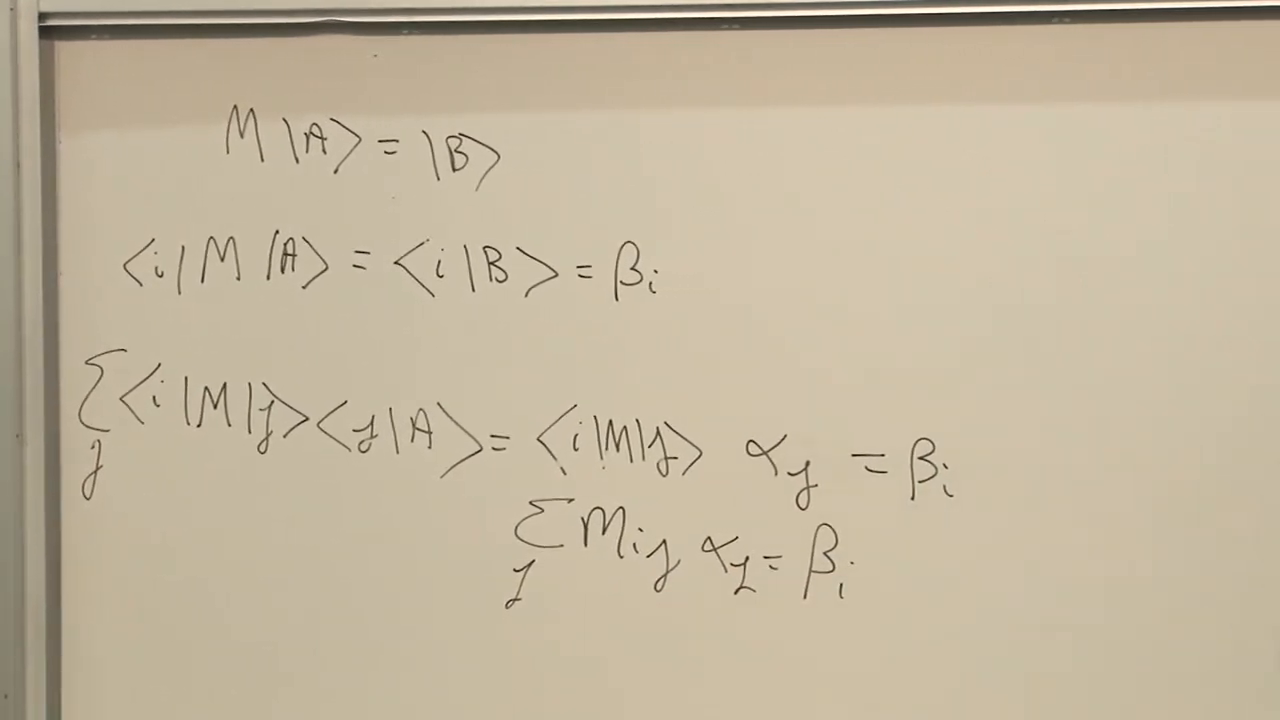
\includegraphics[width=0.84\textwidth]{lecture_03_figure_02.png}
\caption{將抽象方程\(M\ket{A}=\ket{B}\)投影並展開後，得到分量形式的規則\(\sum_jm_{ij}\alpha_j=\beta_i\)。}
\lectureframe{00:18:30}
\end{figure}

若空間的維度為\(N\)，則\(N^2\)個數值\(m_{ij}\)構成一個\(N\times N\)方陣。式~\eqref{eq:component-action}正是
\begin{equation}
\begin{pmatrix}
m_{11}&m_{12}&\cdots&m_{1N}\\
m_{21}&m_{22}&\cdots&m_{2N}\\
\vdots&\vdots&\ddots&\vdots\\
m_{N1}&m_{N2}&\cdots&m_{NN}
\end{pmatrix}
\begin{pmatrix}
\alpha_1\\
\alpha_2\\
\vdots\\
\alpha_N
\end{pmatrix}
=
\begin{pmatrix}
\beta_1\\
\beta_2\\
\vdots\\
\beta_N
\end{pmatrix}.
\label{eq:matrix-vector-action}
\end{equation}
要求出\(\beta_1\)，只要用輸入欄向量乘上第一列並加總；求\(\beta_2\)時則用第二列，依此類推。這個矩陣就是惠勒所說機器的具體表示。

\begin{figure}[htbp]
\centering
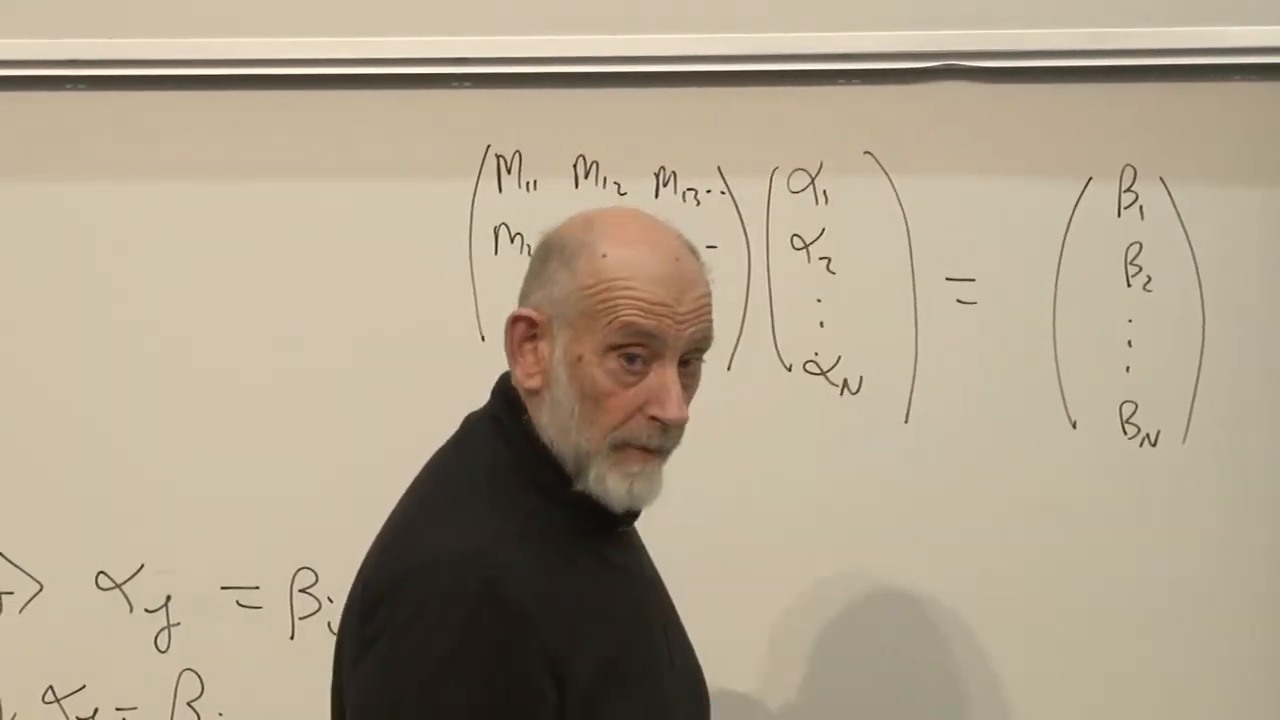
\includegraphics[width=0.84\textwidth]{lecture_03_figure_03.png}
\caption{同一個算符作用，以方陣乘上輸入係數欄向量表示。}
\lectureframe{00:20:01}
\end{figure}

我們得到了一套計算方法，卻也失去部分直觀可見的幾何結構。抽象關係\(M\ket{A}=\ket{B}\)不依賴座標；具體的矩陣元\(m_{ij}\)、\(\alpha_j\)和\(\beta_i\)則取決於所選基底。換用另一組正交歸一基底，這三組數值都會改變，但底層映射及其物理預測不變。

\begin{classroomqa}
\audiencequestion{基底的選擇會決定一道題能不能解嗎？}
\lecturerresponse{基底的選擇會影響解答是否容易看出來。選得恰當，算符可能呈對角形式，計算也幾乎立刻完成；選得不合適，結構則可能被繁瑣的代數運算掩蓋。但基底不能改變實驗結果。若兩種基底導出不同的物理答案，表示計算有誤。}
\end{classroomqa}

\section{左矢、右矢與反線性}

\begin{classroomqa}
\audiencequestion{線性算符能把右矢變成左矢，或把左矢變成右矢嗎？}
\lecturerresponse{剛才定義的一般線性算符不能。它將右矢映射為右矢，而且複數純量通過時保持不變。交換左矢與右矢的運算還會對係數取複共軛，因此屬於另一類運算。}
\end{classroomqa}

乘以固定複數是簡單的線性算符；複共軛則不是。若以\(K\)表示共軛，則
\[
K\bigl(z\ket{A}\bigr)=z^*K\ket{A},
\]
而不是\(zK\ket{A}\)。這類映射稱為\emph{反線性}。這個名稱並非表示它與線性相反，而是指出它會對純量取複共軛。它與反粒子之間更深的關聯，超出本節的討論範圍。

不過，線性算符也能作用於左矢。依照慣例，算符寫在右側：
\begin{equation}
\bra{A}M.
\end{equation}
這樣定義，是為了讓矩陣元的括號不致產生歧義：
\begin{equation}
\bra{A}\bigl(M\ket{B}\bigr)
=
\bigl(\bra{A}M\bigr)\ket{B}
\equiv
\bra{A}M\ket{B}.
\label{eq:bracket-independence}
\end{equation}

展開兩個向量，就能看出這為何可行：
\begin{align}
\bra{A}M\ket{B}
 &=\left(\sum_i\alpha_i^*\bra{i}\right)
   M
   \left(\sum_j\beta_j\ket{j}\right)\\
 &=\sum_{ij}\alpha_i^*m_{ij}\beta_j.
\label{eq:matrix-element-double-sum}
\end{align}
這是一個普通的雙重求和。我們可以先對\(j\)求和，將\(M\)視為作用在右矢上；也可以先對\(i\)求和，將它視為作用在左矢上。兩種方式所得結果相同。這種記號正是為了避免不必要的括號而設計的。

\section{伴隨運算}

另一個相關但不同的問題是：算符如何作用在左矢上？假設
\[
M\ket{A}=\ket{B}.
\]
什麼算符能將相應的左矢\(\bra{A}\)變成\(\bra{B}\)？一般來說，這個算符不是\(M\)本身。若\(M\)是乘以複數\(z\)，右矢方程會是\(\ket{B}=z\ket{A}\)，但左矢方程則會是\(\bra{B}=z^*\bra{A}\)。

所需的算符記為\(M^\dagger\)，稱為\(M\)的\emph{厄米共軛}，定義如下：
\begin{equation}
M\ket{A}=\ket{B}
\quad\Longleftrightarrow\quad
\bra{A}M^\dagger=\bra{B}.
\label{eq:dagger-definition}
\end{equation}
伴隨運算是複共軛在算符上的類比。

其矩陣規則可直接推得。令
\[
M\ket{i}=\ket{i'}.
\]
則
\[
m_{ji}=\bra{j}M\ket{i}=\braket{j}{i'}.
\]
取伴隨後的左矢關係為\(\bra{i}M^\dagger=\bra{i'}\)，所以
\[
(m^\dagger)_{ij}
=\bra{i}M^\dagger\ket{j}
=\braket{i'}{j}.
\]
交換內積兩項的順序，會使內積取複共軛：
\[
\braket{i'}{j}=\braket{j}{i'}^*.
\]
因此
\begin{equation}
\boxed{(m^\dagger)_{ij}=m_{ji}^*.}
\label{eq:dagger-matrix-elements}
\end{equation}

\begin{figure}[htbp]
\centering
\includegraphics[width=0.84\textwidth]{lecture_03_figure_05.png}
\caption{厄米共軛關係的完整板書結果：交換指標並取複共軛。}
\lectureframe{00:42:23}
\end{figure}

用矩陣表示，就是先轉置，再取複共軛：
\begin{equation}
\begin{pmatrix}
a&b\\
c&d
\end{pmatrix}^{\!\dagger}
=
\begin{pmatrix}
a^*&c^*\\
b^*&d^*
\end{pmatrix}.
\label{eq:dagger-two-by-two}
\end{equation}
轉置會使矩陣元相對於主對角線互換位置；取共軛則會將每個\(i\)換成\(-i\)。例如：
\begin{equation}
\begin{pmatrix}
2&6+7i\\
4-i&9+i
\end{pmatrix}^{\!\dagger}
=
\begin{pmatrix}
2&4+i\\
6-7i&9-i
\end{pmatrix}.
\label{eq:dagger-numerical-example}
\end{equation}
對角線上的元素留在原位但取複共軛，兩個非對角元素則互換位置並取複共軛。

\section{厄米算符}

複數等於自身的複共軛，當且僅當它是實數。算符的對應條件也很直接。

\begin{definition}
算符\(M\)稱為\emph{厄米算符}，若
\begin{equation}
M=M^\dagger.
\label{eq:hermitian-definition}
\end{equation}
等價地，在任何正交歸一基底中，
\begin{equation}
m_{ij}=m_{ji}^*.
\label{eq:hermitian-components}
\end{equation}
\end{definition}

在式~\eqref{eq:hermitian-components}中令\(i=j\)，則
\[
m_{ii}=m_{ii}^*,
\]
因此每個對角元素都是實數。非對角元素則成共軛對，彼此相對於主對角線反射。若其中一個元素為\(4-i\)，與它對應的元素便是\(4+i\)；若其中一個是實數\(5\)，另一個也必為實數。

\begin{figure}[htbp]
\centering
\includegraphics[width=0.78\textwidth]{lecture_03_figure_06.png}
\caption{厄米矩陣示例：對角線上的元素為實數，關於對角線互為共軛的元素成對出現。}
\lectureframe{00:45:43}
\end{figure}

厄米算符之所以重要，是因為它們將用來表示可測量量。在建立這項對應之前，我們需要先了解它們的本徵方向。

\section{本徵向量與本徵方向}

第一次接觸本徵向量時，這部分可能會讓人覺得進度比周遭的物理內容快。這些是標準線性代數概念，並非新的物理假設；若不熟悉，不妨先自行複習定義，再回來繼續推導。

一般算符會改變向量的方向。例如，普通三維空間中的旋轉幾乎會使每個向量都偏離原來的方向。旋轉軸是例外：沿著軸的向量經旋轉後方向不變。這就是本徵向量的典型例子。

實二維平面上的非平凡旋轉，則說明了另一種可能：不存在任何方向，能在乘上實數倍後保持不變。因此，作用於受限實向量空間的一般算符未必有實本徵向量。量子力學所用複數態空間上的厄米算符，則有更強的性質。

\(M\)的本徵向量滿足
\begin{equation}
M\ket{i}=\lambda_i\ket{i}.
\label{eq:eigenvalue-equation}
\end{equation}
數值\(\lambda_i\)稱為本徵值。本徵向量是相對於某個算符而言的；若不指明是哪個映射保持其方向，就不能只談本徵向量。

式~\eqref{eq:eigenvalue-equation}並未固定本徵向量的長度或相位。對任何非零複數\(z\)，
\[
M\bigl(z\ket{i}\bigr)
=zM\ket{i}
=\lambda_i\bigl(z\ket{i}\bigr).
\]
因此，更精確的說法是\emph{本徵方向}：\(\ket{i}\)的任何非零倍數都代表同一方向，也有相同的本徵值。我們通常會選取一個歸一化的代表向量。

譜定理的核心結論是：在一個\(N\)維複數向量空間上，厄米算符有一組由\(N\)個本徵向量構成的完備正交歸一基底。這個結論的兩個部分，只需少量代數便能看出。

\subsection{厄米算符的本徵值為實數}

假設\(M=M^\dagger\)，且
\[
M\ket{i}=\lambda_i\ket{i}.
\]
對整個方程取厄米共軛：
\begin{equation}
\bra{i}M^\dagger=\lambda_i^*\bra{i}.
\label{eq:eigen-bra-equation}
\end{equation}
由於\(M^\dagger=M\)，分別將右矢方程從左側乘上\(\bra{i}\)，以及將左矢方程從右側乘上\(\ket{i}\)：
\begin{align}
\bra{i}M\ket{i}&=\lambda_i\braket{i}{i},\\
\bra{i}M\ket{i}&=\lambda_i^*\braket{i}{i}.
\end{align}
兩個數值都乘上同一個非零範數，因此
\begin{equation}
\lambda_i=\lambda_i^*.
\end{equation}
厄米算符的本徵值全為實數。這初步顯示，厄米算符可以表示測量儀器所顯示的實數。

\subsection{不同本徵值對應的本徵向量彼此正交}

令
\[
M\ket{i}=\lambda_i\ket{i},
\qquad
M\ket{j}=\lambda_j\ket{j},
\]
其中\(M\)是厄米算符。對第二個方程取厄米共軛。已知其本徵值為實數：
\[
\bra{j}M=\lambda_j\bra{j}.
\]
接著將第一個方程從左側乘上\(\bra{j}\)，並將左矢方程從右側乘上\(\ket{i}\)：
\begin{align}
\bra{j}M\ket{i}&=\lambda_i\braket{j}{i},\\
\bra{j}M\ket{i}&=\lambda_j\braket{j}{i}.
\end{align}
兩式相減，得到
\begin{equation}
\boxed{(\lambda_i-\lambda_j)\braket{j}{i}=0.}
\label{eq:hermitian-orthogonality}
\end{equation}
若\(\lambda_i\ne\lambda_j\)，則
\[
\braket{j}{i}=0.
\]
兩個本徵方向彼此正交。

\begin{figure}[htbp]
\centering
\includegraphics[width=0.82\textwidth]{lecture_03_figure_07.png}
\caption{正交性證明中的關鍵一步：本徵值不相等，便迫使內積為零。}
\lectureframe{00:59:00}
\end{figure}

若兩個本徵值相同，式~\eqref{eq:hermitian-orthogonality}便不會對該簡併本徵空間內的向量施加任何限制。我們可以在其中選取一組正交歸一基底。這些向量再與其他本徵方向合在一起，就構成譜定理所保證的完備正交歸一本徵基底。

正交性也有物理上的意義。透過適當的測量，可以毫無歧義地區分兩個正交態。不同本徵值的本徵態必定可區分，因為儀器會對它們顯示不同的實數。代數結果與可操作的物理意義，已指向同一項對應關係。

\section{測量公設}

現在我們已有足夠的數學架構，可以陳述量子力學的基本對應關係。初次接觸時，這些關係或許顯得陌生；唯有實際運用後，意義才會具體呈現。因此，我們先清楚列出它們，再立刻回到自旋實驗。

一次測量會得到一個實數。兩個相容的實數讀值可以合併表示成一個複數，但那仍包含兩次測量的結果。單一探測器的基本讀值是實數。因此，厄米算符是自然的候選者：它們的本徵值是實數，本徵向量則構成完備正交歸一基底。

\begin{enumerate}
\item 可測量量，或稱\emph{可觀測量}，以厄米算符\(M\)表示。
\item 測量\(M\)可能得到的結果，是其本徵值\(\lambda_i\)。
\item 若一個態中的\(M\)具有確定值\(\lambda_i\)，則該態是滿足下式的本徵態\(\ket{i}\)：
\[
M\ket{i}=\lambda_i\ket{i}.
\]
\item 若系統處於一般的歸一化態\(\ket{A}\)，得到\(\lambda_i\)的機率為
\begin{equation}
P(\lambda_i\mid A)
=\left|\braket{i}{A}\right|^2
=\braket{i}{A}\braket{A}{i}.
\label{eq:born-rule}
\end{equation}
\end{enumerate}

這份列表是方便的起點，但未必是最精簡的獨立公設系統；採用更精簡的表述時，其中一些陳述可以由其他陳述推導而來。將這些對應關係分開列出，有助於看清各自的物理作用。

複數\(\braket{i}{A}\)是\emph{機率振幅}，而不是機率。將它乘上自己的複共軛，就會得到實數且非負的數值。對於自旋分量，其譜只有兩個值：\(+1\)和\(-1\)；更一般的可觀測量則可能有許多本徵值。

\begin{figure}[htbp]
\centering
\includegraphics[width=0.82\textwidth]{lecture_03_figure_08.png}
\caption{板書將確定結果的態與本徵向量連結，並將得到\(\lambda_i\)的機率與投影至\(\ket{i}\)的模平方連結。}
\lectureframe{01:11:29}
\end{figure}

\begin{classroomqa}
\audiencequestion{機率規則中的\(P\)旁邊，究竟寫著什麼？}
\lecturerresponse{寫的是\(\lambda_i\)：\(P(\lambda_i\mid A)\)表示系統製備為\(\ket{A}\)時，測量\(M\)而得到特定本徵值\(\lambda_i\)的機率。右側則是投影至該本徵向量所得振幅的模平方。}
\end{classroomqa}

\subsection{歸一化與完備性}

所有互斥結果的機率總和必須為1：
\begin{equation}
\sum_i\left|\braket{i}{A}\right|^2=1.
\label{eq:probability-normalization}
\end{equation}
將完備本徵基底代入：
\begin{align}
\sum_i\left|\braket{i}{A}\right|^2
 &=\sum_i\braket{A}{i}\braket{i}{A}\\
 &=\bra{A}\left(\sum_i\ket{i}\bra{i}\right)\ket{A}\\
 &=\braket{A}{A}.
\end{align}
因此，可容許的態向量必須歸一化：
\begin{equation}
\braket{A}{A}=1.
\label{eq:state-normalization}
\end{equation}
若\(\ket{A}=\sum_i\alpha_i\ket{i}\)，相同條件可寫成
\begin{equation}
\sum_i\alpha_i^*\alpha_i=1.
\label{eq:component-normalization}
\end{equation}
這是對複數分量的一項實數限制。

\begin{classroomqa}
\audiencequestion{每個機率都必須是正數嗎？}
\lecturerresponse{是。每個機率都等於一個數乘上自己的複共軛，因此必定非負。歸一化條件則使這些數的總和等於1。}
\end{classroomqa}

還有一種冗餘。若將每個分量都乘上相同的相位，
\begin{equation}
\ket{A}\longmapsto e^{i\theta}\ket{A},
\label{eq:l3-global-phase}
\end{equation}
每個振幅都會乘上\(e^{i\theta}\)，但其模平方不變。任何測量都無法測出這個共同相位。分量間的相對相位仍具有物理意義；只有乘在整個態上的整體相位是冗餘的。

因此，任意複數向量中的兩個實參數並不足以決定物理態：態的大小由歸一化條件固定，整體相位則不可觀測。這與單一自旋的參數計數相同，只是現在從一般機率規則推導而來。

\subsection{測量也會製備態}

還有一項公設，用一句話說比寫成一行簡短的板書更容易。若測量得到\(\lambda_i\)，測量後系統便處於相應的本徵態\(\ket{i}\)。儀器不只記錄結果，也會製備出一個態，使得立即重複同一測量時，結果必定確定。

\begin{classroomqa}
\audiencequestion{能再說一次測量會製備態這項陳述嗎？}
\lecturerresponse{測量前，依照式~\eqref{eq:born-rule}所列的機率，可能得到不同本徵值。一旦儀器實際測得\(\lambda_i\)，系統便處於對應於\(\lambda_i\)的本徵態。因此，立刻再次測量同一可觀測量，會得到相同的值。}
\end{classroomqa}

\begin{classroomqa}
\audiencequestion{這些原理已經告訴我們態如何隨時間演化了嗎？}
\lecturerresponse{還沒有。我們已經說明態是什麼、可觀測量如何表示，以及測量會造成什麼結果。描述系統如何隨時間變化的定律屬於額外架構，稍後才會引入。這就像先定義經典相空間，再寫下運動方程。}
\end{classroomqa}

\begin{classroomqa}
\audiencequestion{先前討論自旋沿傾斜軸的平均值時，出現了\(\cos\theta\)。現在有了振幅模平方規則，平均值是不是應該變成\(\cos^2\theta\)？}
\lecturerresponse{機率與平均值是不同的量。平均值要將\(+1\)與\(-1\)兩種結果的機率，連同各自的正負號一起計算。建構出任意方向的自旋態後，振幅的模平方會導出先前得到的餘弦平均值。這是接下來要做的推導，不應靠改動舊公式來猜。}
\end{classroomqa}

\section{自旋：第一個應用}

三個可測量的自旋分量以厄米算符表示：
\[
\sigma_x,\qquad \sigma_y,\qquad \sigma_z.
\]
分析器實驗已經給出它們的可能值，以及具有確定值的態：
\[
\begin{array}{c|c|c}
\text{observable}&\text{eigenvalue }+1&\text{eigenvalue }-1\\ \hline
\sigma_z&\ket{u}&\ket{d}\\
\sigma_x&\ket{r}&\ket{l}\\
\sigma_y&\ket{\mathrm{in}}&\ket{\mathrm{out}}
\end{array}
\]
這些資訊足以將算符重建為矩陣。

\subsection{在本徵基底中表示 z 分量}

選用上--下基底。自旋沿\(z\)方向具有確定值，表示
\begin{equation}
\sigma_z\ket{u}=+\ket{u},
\qquad
\sigma_z\ket{d}=-\ket{d}.
\label{eq:sigma-z-eigenvectors}
\end{equation}
兩個本徵值不同，因此由厄米性可知\(\braket{u}{d}=0\)。

計算四個矩陣元：
\begin{align}
\bra{u}\sigma_z\ket{u}&=+1,&
\bra{u}\sigma_z\ket{d}&=-\braket{u}{d}=0,\\
\bra{d}\sigma_z\ket{u}&=\braket{d}{u}=0,&
\bra{d}\sigma_z\ket{d}&=-1.
\end{align}
因此
\begin{equation}
\boxed{
\sigma_z=
\begin{pmatrix}
1&0\\
0&-1
\end{pmatrix}_{\{u,d\}}.}
\label{eq:sigma-z}
\end{equation}
座標欄向量為
\[
\ket{u}\widehat{=}\begin{pmatrix}1\\0\end{pmatrix},
\qquad
\ket{d}\widehat{=}\begin{pmatrix}0\\1\end{pmatrix}.
\]
將式~\eqref{eq:sigma-z}所示的矩陣作用在欄向量上，第一欄保持不變，第二欄則變號，恰好符合本徵值方程。

\begin{figure}[htbp]
\centering
\includegraphics[width=0.82\textwidth]{lecture_03_figure_09.png}
\caption{在上--下基底中，\(\sigma_z\)的本徵值方程及其對角矩陣。}
\lectureframe{01:26:56}
\end{figure}

\subsection{固定基底求 x 分量}

在右--左基底中，\(\sigma_x\)會呈現相同的對角形式。這樣算雖然簡單，卻看不出多少東西。我們保留上--下基底，並使用
\begin{equation}
\sigma_x\ket{r}=+\ket{r},
\qquad
\sigma_x\ket{l}=-\ket{l}.
\label{eq:sigma-x-eigenvectors}
\end{equation}
兩組基底之間的關係為
\begin{align}
\ket{r}&=\frac{\ket{u}+\ket{d}}{\sqrt2},&
\ket{l}&=\frac{\ket{u}-\ket{d}}{\sqrt2},\\
\ket{u}&=\frac{\ket{r}+\ket{l}}{\sqrt2},&
\ket{d}&=\frac{\ket{r}-\ket{l}}{\sqrt2}.
\label{eq:x-z-basis-relations}
\end{align}

先計算左上方的對角元素：
\begin{align}
\bra{u}\sigma_x\ket{u}
 &=\frac12(\bra{r}+\bra{l})\sigma_x(\ket{r}+\ket{l})\\
 &=\frac12(\bra{r}+\bra{l})(\ket{r}-\ket{l})\\
 &=0.
\end{align}
右態與左態彼此正交歸一，因此兩個對角項相消，交叉項也為零。對\(\ket{d}\)進行同樣的計算，可得
\[
\bra{d}\sigma_x\ket{d}=0.
\]
此時兩個零並不表示算符為零；這表示我們該轉而計算非對角元素。

右上方的矩陣元為
\begin{align}
\bra{u}\sigma_x\ket{d}
 &=\frac12(\bra{r}+\bra{l})\sigma_x(\ket{r}-\ket{l})\\
 &=\frac12(\bra{r}+\bra{l})(\ket{r}+\ket{l})\\
 &=1.
\end{align}
利用厄米性，或直接重做一次計算，可得
\[
\bra{d}\sigma_x\ket{u}=1.
\]
因此
\begin{equation}
\boxed{
\sigma_x=
\begin{pmatrix}
0&1\\
1&0
\end{pmatrix}_{\{u,d\}}.}
\label{eq:sigma-x}
\end{equation}
同一個抽象算符在自己的本徵基底中呈對角形式，在\(z\)基底中則呈非對角形式。這具體說明了矩陣表示雖會隨基底改變，物理上卻沒有歧義。

\subsection{y 分量與相對相位}

採用以下歸一化的入--出態慣例：
\begin{equation}
\ket{\mathrm{in}}=\frac{\ket{u}+i\ket{d}}{\sqrt2},
\qquad
\ket{\mathrm{out}}=\frac{\ket{u}-i\ket{d}}{\sqrt2},
\label{eq:l3-in-out-states}
\end{equation}
其中
\[
\sigma_y\ket{\mathrm{in}}=+\ket{\mathrm{in}},
\qquad
\sigma_y\ket{\mathrm{out}}=-\ket{\mathrm{out}}.
\]
互換標籤或反轉\(y\)軸，只會改變符號慣例，不會改變底層構造。利用式~\eqref{eq:l3-in-out-states}，以這兩個本徵向量及其本徵值為條件，可得唯一的厄米矩陣：
\begin{equation}
\boxed{
\sigma_y=
\begin{pmatrix}
0&-i\\
i&0
\end{pmatrix}_{\{u,d\}}.}
\label{eq:sigma-y}
\end{equation}
只需驗算，不必重新推導：
\begin{align}
\begin{pmatrix}0&-i\\i&0\end{pmatrix}
\frac1{\sqrt2}\begin{pmatrix}1\\i\end{pmatrix}
&=\frac1{\sqrt2}\begin{pmatrix}1\\i\end{pmatrix},\\
\begin{pmatrix}0&-i\\i&0\end{pmatrix}
\frac1{\sqrt2}\begin{pmatrix}1\\-i\end{pmatrix}
&=-\frac1{\sqrt2}\begin{pmatrix}1\\-i\end{pmatrix}.
\end{align}
因子\(1/\sqrt2\)用來將本徵向量歸一化，但不影響其本徵方向。

\begin{figure}[htbp]
\centering
\includegraphics[width=0.82\textwidth]{lecture_03_figure_10.png}
\caption{在上--下基底中完整列出的泡利矩陣。}
\lectureframe{01:38:11}
\end{figure}

\begin{classroomqa}
\audiencequestion{入--出態中的一個符號是否應該改變，才能使兩態正交？}
\lecturerresponse{不必。關鍵是把右矢轉成左矢時要取複共軛：
\[
\bra{\mathrm{in}}=\frac{\bra{u}-i\bra{d}}{\sqrt2}.
\]
因此
\[
\begin{aligned}
\braket{\mathrm{in}}{\mathrm{out}}
&=\frac12(\bra{u}-i\bra{d})
  (\ket{u}-i\ket{d})\\
&=\frac12\bigl(1+(-i)(-i)\bigr)\\
&=0.
\end{aligned}
\]
忘了取共軛，正是左矢--右矢記號要揭示的常見錯誤。}
\end{classroomqa}

我們已經得到
\begin{equation}
\begin{aligned}
\sigma_x&=\begin{pmatrix}0&1\\1&0\end{pmatrix},\\[0.4em]
\sigma_y&=\begin{pmatrix}0&-i\\i&0\end{pmatrix},\\[0.4em]
\sigma_z&=\begin{pmatrix}1&0\\0&-1\end{pmatrix}.
\end{aligned}
\label{eq:pauli-triple}
\end{equation}
這些算符都是厄米的，本徵值為\(\pm1\)，而且具有分析器實驗所要求的確定自旋本徵態。

接下來要處理的問題已經明確：給定一個沿任意方向製備的自旋，如何建構相應的態，並利用振幅的模平方計算\(\sigma_z=+1\)和\(\sigma_z=-1\)的機率？現有形式架構提供了足夠資訊；接著自然就該完成這項計算。
